% This file was created by matplotlib2tikz v0.6.17.
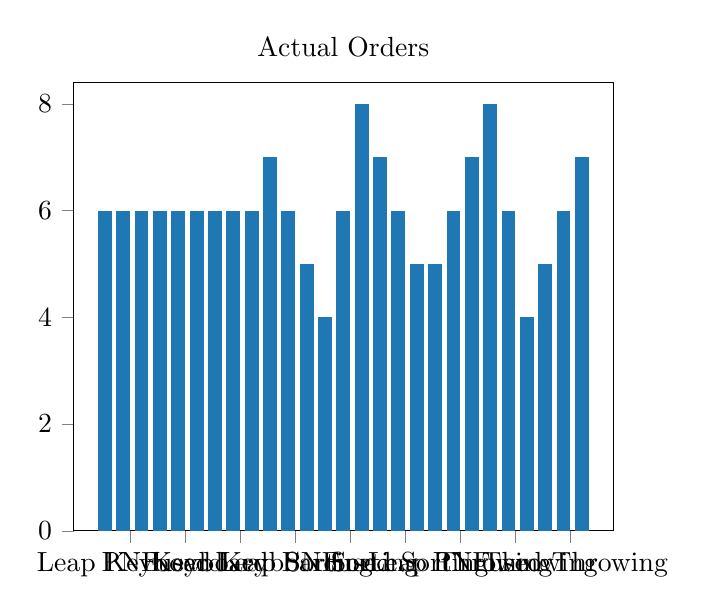
\begin{tikzpicture}

\definecolor{color0}{rgb}{0.12156862745098,0.466666666666667,0.705882352941177}

\begin{axis}[
title={Actual Orders},
xmin=-2.28333333333333, xmax=36.95,
ymin=0, ymax=8.4,
xtick={1.83333333333333,5.83333333333333,9.83333333333333,13.8333333333333,17.8333333333333,21.8333333333333,25.8333333333333,29.8333333333333,33.8333333333333},
xticklabels={Leap
Keyboard,PN
Keyboard,Fused
Keyboard,Leap
Sorting,PN
Sorting,Fused
Sorting,Leap
Throwing,PN
Throwing,Fused
Throwing},
tick align=outside,
tick pos=left,
x grid style={white!69.019607843137251!black},
y grid style={white!69.019607843137251!black}
]
\draw[fill=color0,draw opacity=0] (axis cs:-0.5,0) rectangle (axis cs:0.5,6);
\draw[fill=color0,draw opacity=0] (axis cs:0.833333333333333,0) rectangle (axis cs:1.83333333333333,6);
\draw[fill=color0,draw opacity=0] (axis cs:2.16666666666667,0) rectangle (axis cs:3.16666666666667,6);
\draw[fill=color0,draw opacity=0] (axis cs:3.5,0) rectangle (axis cs:4.5,6);
\draw[fill=color0,draw opacity=0] (axis cs:4.83333333333333,0) rectangle (axis cs:5.83333333333333,6);
\draw[fill=color0,draw opacity=0] (axis cs:6.16666666666667,0) rectangle (axis cs:7.16666666666667,6);
\draw[fill=color0,draw opacity=0] (axis cs:7.5,0) rectangle (axis cs:8.5,6);
\draw[fill=color0,draw opacity=0] (axis cs:8.83333333333333,0) rectangle (axis cs:9.83333333333333,6);
\draw[fill=color0,draw opacity=0] (axis cs:10.1666666666667,0) rectangle (axis cs:11.1666666666667,6);
\draw[fill=color0,draw opacity=0] (axis cs:11.5,0) rectangle (axis cs:12.5,7);
\draw[fill=color0,draw opacity=0] (axis cs:12.8333333333333,0) rectangle (axis cs:13.8333333333333,6);
\draw[fill=color0,draw opacity=0] (axis cs:14.1666666666667,0) rectangle (axis cs:15.1666666666667,5);
\draw[fill=color0,draw opacity=0] (axis cs:15.5,0) rectangle (axis cs:16.5,4);
\draw[fill=color0,draw opacity=0] (axis cs:16.8333333333333,0) rectangle (axis cs:17.8333333333333,6);
\draw[fill=color0,draw opacity=0] (axis cs:18.1666666666667,0) rectangle (axis cs:19.1666666666667,8);
\draw[fill=color0,draw opacity=0] (axis cs:19.5,0) rectangle (axis cs:20.5,7);
\draw[fill=color0,draw opacity=0] (axis cs:20.8333333333333,0) rectangle (axis cs:21.8333333333333,6);
\draw[fill=color0,draw opacity=0] (axis cs:22.1666666666667,0) rectangle (axis cs:23.1666666666667,5);
\draw[fill=color0,draw opacity=0] (axis cs:23.5,0) rectangle (axis cs:24.5,5);
\draw[fill=color0,draw opacity=0] (axis cs:24.8333333333333,0) rectangle (axis cs:25.8333333333333,6);
\draw[fill=color0,draw opacity=0] (axis cs:26.1666666666667,0) rectangle (axis cs:27.1666666666667,7);
\draw[fill=color0,draw opacity=0] (axis cs:27.5,0) rectangle (axis cs:28.5,8);
\draw[fill=color0,draw opacity=0] (axis cs:28.8333333333333,0) rectangle (axis cs:29.8333333333333,6);
\draw[fill=color0,draw opacity=0] (axis cs:30.1666666666667,0) rectangle (axis cs:31.1666666666667,4);
\draw[fill=color0,draw opacity=0] (axis cs:31.5,0) rectangle (axis cs:32.5,5);
\draw[fill=color0,draw opacity=0] (axis cs:32.8333333333333,0) rectangle (axis cs:33.8333333333333,6);
\draw[fill=color0,draw opacity=0] (axis cs:34.1666666666667,0) rectangle (axis cs:35.1666666666667,7);
\end{axis}

\end{tikzpicture}